\chapter{The Control Flow Graph}
\label{chap:CFGConstruction}
In this chapter we give examples of how we recursively generate the CFG of some essential language features, during this we will present the CFG nodes\footnote{The complete list of our CFG nodes can be found in \autoref{chapter:NodeRef}} that we use, together with their semantics.


\section{An example: For loops}
\label{sec:CFGConstructionLoops}
Loops in Python differ from loops in most other languages as both \inlinecode{for} and \inlinecode{while} loops have an \inlinecode{else} branch, as can be seen in \autoref{code:forExample}. The \inlinecode{else} branch is executed if the loop terminates normally, i.e. not using the \inlinecode{break} statement.

\begin{listing}[H]
  \begin{minted}[linenos]{python}
for x in [1,2,3]:
  if (x > 2):
    break
  print x
else:
  print "normal for termination"
  \end{minted}
  \caption{\inlinecode{for} loop example with an \inlinecode{else} block.}\label{code:forExample}
\end{listing}

The semantics is as follows: First, the expression given to the loop, \inlinecode{[1,2,3]}, is evaluated. This should result in an iterable object, such that an iterator object can be created. For each element in the iterator the body of the loop is evaluated.

To simulate this in our CFG we need to take a look at the iterator object: to get the next element from an iterator object the \inlinecode{next} method is called. This method returns the next element until the iteration is done and finally raises a \inlinecode{StopIteration} exception.

The generated CFG for \autoref{code:forExample} can been seen in \autoref{fig:forCfg}.

\begin{figure}{H}
  \begin{center}
    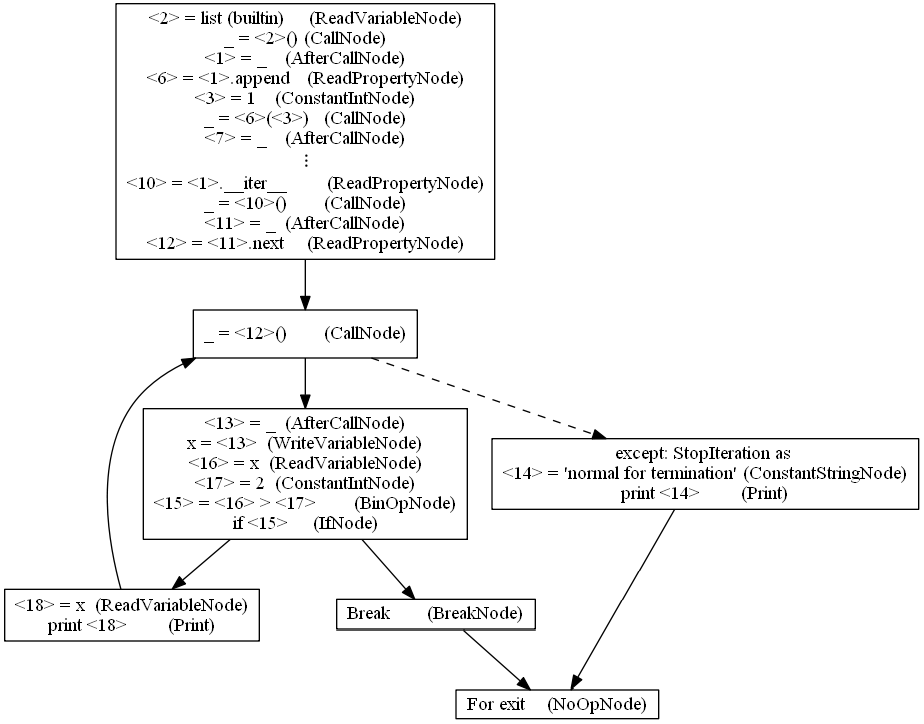
\includegraphics[width=0.85\textwidth]{images/for-example-cfg2.png}
  \end{center}
  \caption{CFG for the for-loop \autoref{code:forExample}.}
  \label{fig:forCfg}
\end{figure}


\section{Using registers for the intermediate representation}
\label{CFG calls}
Inspired from TAJS \cite{tajs} we use registers in our intermediate representation to model that even simple expressions in Python is evaluated in several steps. To illustrate this consider the following line of code from \autoref{code:Features1}: \inlinecode{s1.addGrade('math', 10)}.

First the function \inlinecode{addGrade} is looked up in the class of \inlinecode{s1}. This is done in the CFG using \textit{ReadAttributeNode}, which holds a result register, a base register (i.e. the register where to find the object), and the name of the attribute to look up. Similar nodes include \textit{ReadVariableNode} and \textit{ReadIndexableNode}.

\begin{figure}{H}
	\begin{center}
		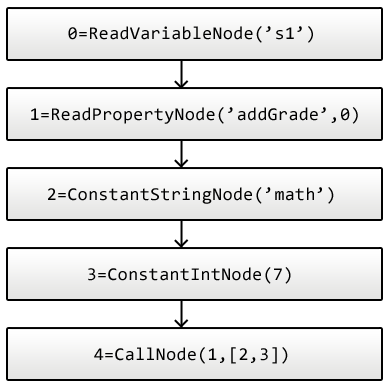
\includegraphics[width=0.35\textwidth]{images/Call-example.png}
	\end{center}
	\caption{CFG for a call example.}
	\label{fig:callCfg}
\end{figure}

Second, each argument given to the function is evaluated and stored in individual registers, and finally the actual call can be made. Calls in the CFG is modeled using the \textit{CallNode}, which holds a function register and a list of argument registers, and \textit{AfterCallNode}, which holds a result register.

Thus the expression \inlinecode{s1.addGrade('math', 10)} will result in the CFG found in \autoref{fig:callCfg} 
(where the numbers to the left represent the result registers of the nodes).

So far we have primarily been concerned with putting constants into registers and reading variables and attributes. In order to support writing we have three different nodes: \textit{WriteVariableNode}, \textit{WriteAttributeNode}, and \textit{WriteIndexableNode}. Besides holding a value register, i.e. the register where to find the value being written, \textit{WriteVariableNode} contains the name of the variable being written to, \textit{WriteAttributeNode} contains a base register and the attribute being written to, and \textit{WriteIndexableNode} contains a base and attribute register (the latter has a register for the attribute because it is not constant, for instance we could write something like the following: \inlinecode{dict[getKey()] = aValue}, whereas attribute in \inlinecode{obj.attribute = aValue} must be a string).



\section{Magic methods}
The so-called magic methods can be thought of as hooks, which allow the programmer to get to execute code at attribute access and other similar places. This is something that cannot be done in JavaScript.

From a static analysis point of view some of these magic methods are less interesting. For instance the magic method \inlinecode{\_\_init\_\_} just corresponds to a constructor.

\begin{sloppypar}
However, two very interesting magic methods are \inlinecode{\_\_getattribute\_\_} and \inlinecode{\_\_getattr\_\_}, because each time an attribute \inlinecode{a} is read from a class instance \inlinecode{x}, the following happens:
\end{sloppypar}

The magic method \inlinecode{\_\_getattribute\_\_} is looked up on \inlinecode{x}. If it is defined by the programmer, the method is called with the instance, \inlinecode{x}, and the attribute name \inlinecode{a}. It is now up to the supplied method to return the correct value\footnote{For instance the implementation of \inlinecode{\_\_getattribute\_\_} could just return a constant, which would cause every attribute access to result in that particular constant.}. If the implementation of \inlinecode{\_\_getattribute\_\_} happens to raise an \inlinecode{AttributeError}, \inlinecode{\_\_getattr\_\_} is called. Otherwise if \inlinecode{\_\_getattribute\_\_} is not defined, the attribute is looked up on the instance. If the attribute is present on the instance it is returned, otherwise an \inlinecode{AttributeError} is raised and the magic method \inlinecode{\_\_getattr\_\_} is called if it is defined.

The following pseudo code should clarify this:

\begin{listing}[H]
  \begin{minted}[linenos]{python}
def readAttribute(x,a):
  __getattribute__ = lookup(x,'__getattribute__')
  __getattr__ = lookup(x,'__getattr__')

  try:
    if isset(__getattribute__):
      # __getattribute__ is called if defined
      return __getattribute__(x,a)
    else:
      return getattr(x,a)
  except AttributeError as e:
    if isset(__getattr__):
      # __getattr__ called in case of an AttributeError
      return __getattr__(x,a)
    else
      raise e
  \end{minted}
  \caption{Pseudo code to clarify the attribute lookup mechanism.}
\end{listing}

Thus, the magic method \inlinecode{\_\_getattribute\_\_} can be used to supply a custom attribute lookup function, and \inlinecode{\_\_getattr\_\_} can be used to supply a fallback function in case of a bad attribute access. It should also be noted that \inlinecode{\_\_getattribute\_\_} cannot be thought of as being equivalent (or nearly equivalent) to getters in ECMAScript 5 and C\#: In Python one single method is supplied, not one for each attribute.

As mentioned in the introduction we have only aimed to support \inlinecode{\_\_getattr\_\_} in our type analyser, due to the limited time of our project. However, in order to determine that we wanted to support \inlinecode{\_\_getattr\_\_} and not \inlinecode{\_\_getattribute\_\_}, we looked at the use of these magic methods in some larger Python projects. In Django \cite{django}, a high-level web framework, we found that \inlinecode{\_\_getattribute\_\_} was not used at all. However, \inlinecode{\_\_getattr\_\_} is used 14 times and therefore seems more useful to support if the choice stands between the two of them. Of course 14 usages is not much for a web framework on approximately 200.000 lines of code, but it is still essential to handle in order to be able to statically analyse Python programs.

\subsection{Transforming the CFG}
\label{Magic methods transformation}
Since every attribute access possibly involves method calls we normalize the CFG in order to reflect this. More concretely, we normalize each node in the CFG of the following form: \inlinecode{<res>=ReadAttribute(<base>,attr)}, into the following CFG piece:

\begin{listing}[H]
  \begin{center}
    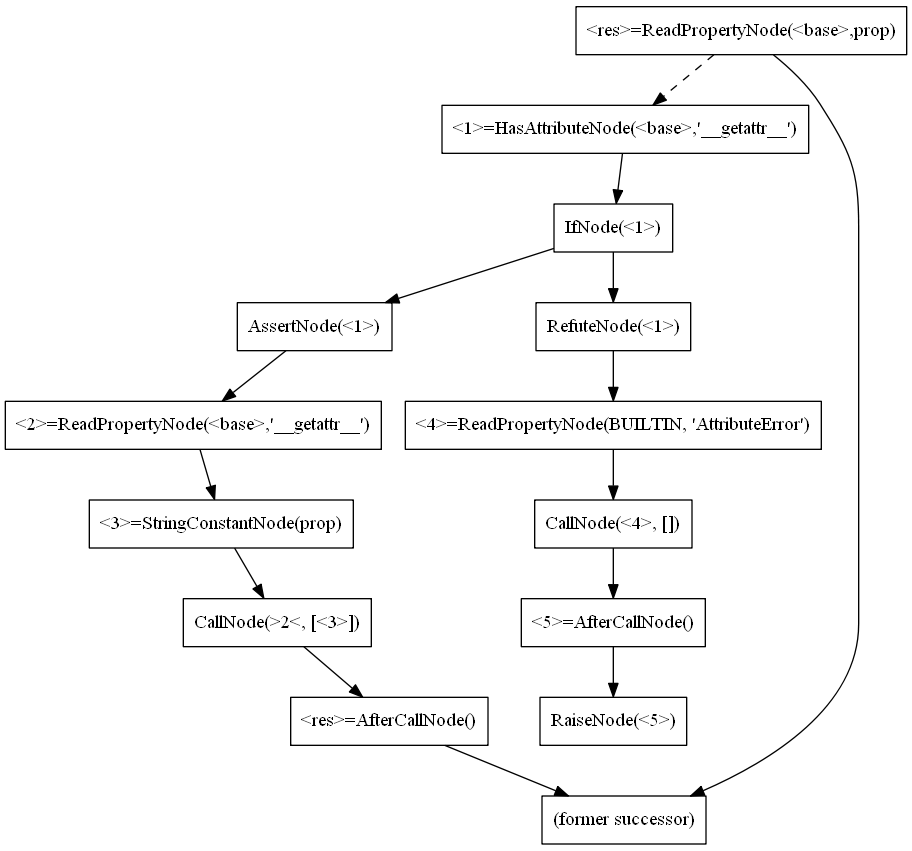
\includegraphics[width=0.9\textwidth]{images/readproperty.png}
  \end{center}
  \vspace{-10pt}
  \caption{The normalization of a read attribute node.}
  \label{fig:MagicMethods1}
\end{listing}

As it can be seen from the normalized CFG for read attribute nodes handling exceptions is key to handling the magic method \inlinecode{\_\_getattr\_\_}. We return to this in the following section, \autoref{chapter:Exceptions}. First, we want to note that if an attribute is \textit{definitely} set on an instance object, \inlinecode{\_\_getattr\_\_} is never called when reading that particular attribute. This is the case as there won't be any flow across the exception edge in the figure above, because the \inlinecode{ReadAttributeNode} will always succeed in reading the attribute and therefore not raise any \inlinecode{AttributeError}. When we can't conclude that an attribute is definitely available read attribute nodes must be normalized (\autoref{ex:DefinitelyAvailable} shows such a scenario).

However, in order for an analysis to conclude that an attribute is definitely set it must support strong updates. We discuss how strong updates can be obtained using recency abstraction in \autoref{section:Strong or weak}. In our current implementation we have no apparent way of making strong updates in a sound fashion. Instead we have introduced a way to tell our analyser that it can assume that allocation-sites only correspond to a single concrete object, thus allowing for strong updates.

\begin{listing}[H]
  \begin{minted}[linenos]{python}
class C():
  if (trickyComputation()):
    C.a = 42
  def __getattr__(self, name):
    return "<bad attribute access>"
x = C()
y = x.a # __getattr__ will be called if trickyComputation() returned false
  \end{minted}
  \caption{In some cases it is not possible to conclude whether an attribute is definitely available or not.}
  \label{ex:DefinitelyAvailable}
\end{listing}

Thus the type analyser can be improved such that it only normalizes read attribute nodes if the attribute being read may not be defined (resulting in possibly $12 * \#\texttt{read attribute nodes}$ nodes less in the CFG)\footnote{...}. This is in fact what our implementation does when we make the assumption previously mentioned. In order to obtain this we have provided the analysis with a hook from the worklist algorithm, such that our type analyser can modify the CFG during the analysis. When doing this each newly added node to the CFG must be added to the worklist.

It is important to note that not supporting \inlinecode{\_\_getattribute\_\_} simplifies the task a bit. Recall that we don't need to normalize read attribute nodes as long the attribute being read is definitely set. This is not the case if we took the magic method \inlinecode{\_\_getattribute\_\_} into account, as it might itself raise an \inlinecode{AttributeError} (causing \inlinecode{\_\_getattr\_\_} to be called)! Thus a type analysis that also supports \inlinecode{\_\_getattribute\_\_} would for a start actually have to normalize all read attribute nodes where an attribute is dereferenced from an instance that belongs from a class where \inlinecode{\_\_getattribute\_\_} is defined. In some cases it might be possible to conclude that the particular implementation of \inlinecode{\_\_getattribute\_\_} will never raise an \inlinecode{AttributeError}, e.g. when the implementation just returns a constant (see the example below), in which the type analysis doesn't need to normalize the read attribute node.

\begin{listing}[H]
  \begin{minted}[linenos]{python}
class C(object):
  def __getattribute__(self, name):
    return 42
  def __getattr__(self, name):
    return "<bad attribute access>"
x = C()
y = x.a # no attribute access will result in __getattr__ being called
  \end{minted}
  \caption{A simple example of when it will be possible to conclude that \inlinecode{\_\_getattr\_\_} will never be called even though \inlinecode{\_\_getattribute\_\_} is defined.}
  \label{code:MagicMethods2}
\end{listing}



\section{Handling exceptions}
\label{chapter:Exceptions}
In order to handle the flow caused by exceptions we introduce a new kind of edge to the CFG. A solid edge will model normal flow while a dashed edge will model exception flow. 

In Python, exceptions can be caught using a try-except-else-finally block. An except block can be annotated with a number of types, and each try-except-else-finally block may contain an arbitrary number of except blocks. As usual, the else block is evaluated after a normal exit, i.e. when no exceptions were raised inside the try block.

The abstract syntax tree (AST) provided by the Jython parser \cite{jython} has been normalized from a try-except-else-finally block into a try-finally block, which contains a try-except-else block. The normalization is illustrated by \autoref{code:tryExceptBefore} and \autoref{code:tryExceptAfter}:

\begin{listing}[H]
	\begin{minted}[linenos]{python}
try: <try>
except Foo: <except-Foo>
except: <except>
else: <else>
finally: <finally>
	\end{minted}
	\caption{A try-except-else-finally example before normalization.}
  \label{code:tryExceptBefore}
\end{listing}

\begin{listing}[H]
	\begin{minted}[linenos]{python}
try: 
  try: <try>
  except Foo: <except-Foo>
  except: <except>
  else: <else>
finally: <finally>
	\end{minted}
	\caption{A try-except-else-finally example after normalization.}
  \label{code:tryExceptAfter}
\end{listing}

\begin{sloppypar}
  Inductively, CFGs for the statement lists \inlinecode{<try>} (\textit{CFG$_{\textit{try}}$}), 
  \inlinecode{<except-Foo>} (\textit{CFG$_{\textit{except-Foo}}$}), \inlinecode{<except>} (\textit{CFG$_{\textit{except}}$}), 
  \inlinecode{<else>} (\textit{CFG$_{\textit{else}}$}), and \inlinecode{<finally>} are created. 
\end{sloppypar}

The CFG for the finally block is then cloned into three duplicates (\textit{CFG$_{\textit{finally-normal}}$}, 
\textit{CFG$_{\textit{finally-handled-exc}}$}, and \textit{CFG$_{\textit{finally-unhandled-exc}}$}). The purpose is to have one finally block for each of the following cases: 

\begin{enumerate}
  \item when no exceptions occur during the try block,
  \item when an exception is raised and caught by one of the surrounding except blocks, and no exception is raised from inside that except block, and
  \item when an exception is raised but not caught, which is the case when 
    a) an exception is raised from the try block and no except blocks handles this particular exception, 
    b) an except block catches an exception raised by the try block, but then raises a new exception on its own.
\end{enumerate}

In particular, it is important that the finally block handling case (3), \textit{CFG$_{\textit{finally-unhandled-exc}}$}, 
is not connected to the exit node of the try-except-else-finally block (this is illustrated in \autoref{fig:tryExceptAfter})! Instead, it should be connected to its nearest surrounding except block (if any), or no except block at all (indicating that the program crashes with a runtime error because of an unhandled exception).

In the following sections we present the way we generate the CFG of a try-except-else-finally block. In \autoref{chapter:Exceptions} we describe how we handle exceptions in the analysis.


\subsection{The try block}
Each node in \textit{CFG$_{\textit{try}}$} (that does not already have an outgoing exception edge) is connected using an exception edge to the entry node of the first except block (\inlinecode{*}), in this case the entry node of \textit{CFG$_{\textit{except-Foo}}$}. We do not add exception edges to nodes that already have an exception edge, because this would be a loss of information since the control flow always goes to the nearest enclosing except block in case of exceptions.

The above description models if an exception occurs during evaluation of one of the statements in a try block, then the control flow will proceed from the first except block. If there are no except blocks, each node should instead be connected using an exception edge to the entry node of its nearest surrounding except or finally block (specifically \textit{CFG$_{\textit{finally-unhandled-exc}}$}). However, we don't add any exception edges here; these will be added inductively because of (\inlinecode{*}) in case there are any surrounding except or finally blocks.

\begin{figure}{H}
  \begin{center}
    \includegraphics[width=0.48\textwidth]{images/Try-except-else-finally.png}
  \end{center}
  \caption{CFG for try try-except \autoref{code:tryExceptAfter}}
  \label{fig:forCfg}
\end{figure}

\subsection{The except block}
The entry node of each except block is connected using an exception edge to the entry node of the next except block (except for the last block). Thus we make an exception edge from the entry node of \textit{CFG$_{\textit{except-Foo}}$} to the entry node of \textit{CFG$_{\textit{except}}$}.

We do this because the first except block might not catch the exception, due to the type restrictions, in which the control flow proceeds to the next except block.

Furthermore, each node inside the except block should be connected using an exception edge to the entry node of its nearest surrounding except or finally block (specifically \textit{CFG$_{\textit{finally-unhandled-exc}}$}). Again, this is handled inductively.

Finally, if an except block actually catches the exception and no exceptions occur inside that except block, the control flow proceeds to the surrounding finally block (in this case, \textit{CFG$_{\textit{finally-handled-exc}}$}). 



\subsection{The else block}
If no exceptions occur the else block should be evaluated. To model this we add a normal flow edge from the exit node of \textit{CFG$_{\textit{try}}$} to the entry node of \textit{CFG$_{\textit{else}}$}.

Since exceptions may result from evaluating the else block, each node in \textit{CFG$_{\textit{else}}$} should also be connected by an exception edge to the entry node of the nearest surrounding except or finally block (again, \textit{CFG$_{\textit{finally-unhandled-exc}}$}).

If the evaluation of the else block does not raise any exceptions, the control flow proceeds either to the exit node of the whole try-except-else block, or in case there is a surrounding finally block, to the entry node of \textit{CFG$_{\textit{finally-normal}}$}.



\section{Global Statement}
At first glance the \inlinecode{global} statement in Python seems rater straightforward to analyse, but it has some interesting quirks that are not intuitive, and thus deserves special treatment. In this section we will describe these quirks and how they are handled by the analysis.

The statement allows the programmer to declare a variable global for the entirety of the scope. No matter where the \inlinecode{global} statement is stated within the block it will take effect, including statements that proceed it. It should also be noted that the statement doesn't have to be executed, so \inlinecode{global} statements in dead code also take effect as seen below:

\begin{listing}[H]
  \begin{minted}[linenos]{python}
x = 10
def foo():
  x = 20
  return
  global x
foo() # x = 20
  \end{minted}
  \caption{Global statements take effect even in dead code.}
\end{listing}

When a variable has been declared global all reads and writes of that variable are done directly in the global scope (top-level). This is done without consideration for any scopes that might have been checked first under normal circumstances.

Since the \inlinecode{global} statement only affects the inner most scope, it can always be statically determined which scope the variable is inclosed by. Therefore the global flag on that variable can be strongly updated.

\begin{listing}[H]
  \begin{minted}[linenos]{python}
x = 10
def foo():
  if (trickyComputation()):
    global x
  x = 20
foo()
x # always 20
  \end{minted}
  \caption{A situation that courses trouble for the join function used in the monotone framework.}
\end{listing}

Due to the fact that the \inlinecode{global} statement takes effect no matter where it is in the block, it courses problems for the join function since a situation where a variable \inlinecode{x} is marked as global in one state and not in the other can arise. In such a situation the state where the variable is not marked as global is in principal incorrect, since the global statement changes the variable for the entire scope, so it has to do some fixing to change this. To avoid this problem a postprocessing phase of the CFG is introduced where CFG nodes corresponding to \inlinecode{global} statements are moved to the top of the block. This way the join function can stay the same.


%\section{\inlinecode{with} statements}
%With statements in Python are unlike With statements in JavaScript.\ They are usually used when you have object you need to "open" before you do some work and then "close" it in the end, this pattern is used a lot when working with I/O such as files or databases.\ An example of with statements can be seen in \autoref{code:withExample}.

%\begin{listing}[H]
%  \begin{minted}[linenos]{python}
%with open('file.txt') as fh:
%  print fh.read()
%  \end{minted}
%  \caption{With example reading a file}\label{code:withExample}
%\end{listing}

%The formal description of the With statement can be found in The Python Language Reference compound statement list\cite{pyref.compound} section 7.5, the highlights is that if there is an \inlinecode{as} part of your with statement the result of the method call to \inlinecode{\_\_enter\_\_} assigned to the variable in the with statement. If there is raised an exception during the execution of the body of the With statement it is passed as arguments to the method call \inlinecode{\_\_exit\_\_}, if the result of that call returns something which truth value is \inlinecode{True} the with statement just evaluates normally, If a truth value of \inlinecode{False} is returned the exception isn't caught. If no exceptions happens during execution the \inlinecode{\_\_exit\_\_} method is called, after the body of the With statement, where \inlinecode{None} is passed as arguments.